\documentclass[slidestop,compress,mathserif]{beamer}
%\documentclass[slidestop,compress,mathserif,handout]{beamer}

%\documentclass[xcolor=dvipsnames,handout]{beamer}
%\documentclass[xcolor=dvipsnames]{beamer}

%\documentclass[handout]{beamer}

%%% To get rid of solutions on handouts:
\newcommand{\soln}[1]{\textit{\textcolor{darkGray}{#1}}}				% For slides
%\newcommand{\soln}[1]{ }	% For handouts

% to get pausing to work properly on slides
\newcommand{\hide}[1]{#1}	% For slides
%\newcommand{\hide}[1]{ }	% For handouts


%\usepackage{multicol}
\usepackage{amsfonts}
%\usepackage[pdftex,dvipsnames]{color}
\usepackage{graphicx}
\usepackage{subfigure}
%\usepackage{picinpar}
\usepackage{pifont}
\usepackage{pgf,pgfarrows,pgfnodes}
%\usepackage{wasysym,manfnt,phaistos,empheq}
\usepackage[english]{babel}
\usepackage{pgfpages}
\usepackage{natbib}
\usepackage{hyperref}
\usepackage{multimedia}
%\usepackage{amsfonts,amstext,amssymb,amsbsy,amsopn,amsthm,eucal,latexsym,mathrsfs}
\usepackage{amsmath,amsfonts,amstext,amssymb,amsbsy,amsopn,amsthm,eucal,latexsym,mathrsfs}
\usepackage{ulem}
\usepackage{setspace}
\usepackage{array}
%\usepackage{rotating}
\usepackage{multirow}
\usepackage{verbatim}
\usepackage{multicol}

\setbeamertemplate{navigation symbols}{}

%\usepackage{tikz}
%\usetikzlibrary{arrows,shapes,trees,backgrounds}


%\setbeameroption{show notes on second screen}
%\setbeameroption{show notes}
%\setbeameroption{show only notes}

\definecolor{links}{HTML}{2A1B81}
\hypersetup{colorlinks,linkcolor=,urlcolor=links}

\newtheorem*{principle}{Inscrutibility Principle}
\newtheorem*{punchline}{Punch Line}
\newtheorem{defn}{Definition}

\definecolor{Scarlet}{RGB}{140,17,17}
\definecolor{VassarRed}{RGB}{128,0,0}

% "dinglist" environment
  \renewenvironment{dinglist}[2][blue]
  {\begin{list}{\textcolor{blue}{\ding{#2}}}{}}{\end{list}}
  % Symbol definitions for these lists
  \newcommand{\DingListSymbolA}{43}
  \newcommand{\DingListSymbolB}{243}
  \newcommand{\DingListSymbolC}{224}
  \newcommand{\DingListSymbolD}{219}
  \newcommand{\DingListSymbolCheck}{52}
  \newcommand{\DingListSymbolCross}{56}


  \newenvironment{ballotenv}
{\only{%
\setbeamertemplate{itemize item}{\ding{45}}%
\setbeamertemplate{itemize subitem}{\ding{46}}%
\setbeamertemplate{itemize subsubitem}{\ding{46}}}} {}
\setbeamertemplate{itemize item}{\ding{49}}
\setbeamertemplate{itemize subitem}{\ding{47}}
\setbeamertemplate{itemize subsubitem}{\ding{47}}


%User defined colors: See colors section
\xdefinecolor{oiBlue}{rgb}{0.15, 0.35, 0.55}
\xdefinecolor{gray}{rgb}{0.5, 0.5, 0.5}
\xdefinecolor{darkGray}{rgb}{0.3, 0.3, 0.3}
\xdefinecolor{darkerGray}{rgb}{0.2, 0.2, 0.2}
\xdefinecolor{rubineRed}{rgb}{0.89,0,0.30}
\xdefinecolor{linkCol}{rgb}{0.11,0.49,0.95}	
\xdefinecolor{irishGreen}{rgb}{0,0.60,0}	
\xdefinecolor{darkturquoise}{rgb}{0.44, 0.58, 0.86}
\definecolor{lightGreen}{rgb}{0.533,0.765,0.42}
\xdefinecolor{Regalia}{HTML}{522D80}
\xdefinecolor{ClemsonOrange}{HTML}{EA6A20}

\definecolor{duke@LightGrey}{RGB}{200,200,200}\definecolor{DarkGreen}{RGB}{0,100,0}
\definecolor{Oranges}{RGB}{255,127,0}
\definecolor{LightGray}{RGB}{211,211,211}

%\setbeamertemplate{footline}{%
%  \raisebox{5pt}{\makebox[\paperwidth]{\hfill\makebox[10pt]{\scriptsize\insertframenumber}}}}

\setbeamercolor{equation background}{fg=black,bg=duke@LightGrey}
  % Boxed equation
  \newcommand{\eqbox}[2][0.6]{%
  \centerline{
  \begin{beamerboxesrounded}[lower=equation background,width=#1\hsize,shadow=true]{}
\parbox{#1\hsize}{%
      \[
        \textcolor{black} {#2}
      \]}
  \end{beamerboxesrounded}
}}

\AtBeginSection[] {
  \begin{frame}<beamer>\frametitle{Outline}
    \tableofcontents[currentsection,hideothersubsections]
  \end{frame}
}
%
%
%\AtBeginSubsection[] {
%  \begin{frame}<beamer>\frametitle{Outline}
%    \tableofcontents%[currentsection,currentsubsection]
%  \end{frame}
%}

%\usecolortheme[RGB={82,45,128}]{structure}
%\usecolortheme[RGB={162,80,22}]{structure}
\usecolortheme[RGB={128,0,0}]{structure}
\usetheme[secheader]{Boadilla}
%\usetheme[height=7mm]{Rochester}
%\usetheme{Copenhagen}
%\usetheme{Antibes}
%\usecolortheme{seahorse}
%\usecolortheme{crane}
%\usecolortheme{rose}
%\usefonttheme[onlylarge]{structurebold}
%\usefonttheme[onlymath]{serif}



\def\diag{{\rm diag}}


\def\E{\mathbb{E}}
\def\Prob{\mathbb{P}}
\def\argmin{{\rm argmin}}
\def\argmax{{\rm argmax}}
\def\Def{\stackrel{def}{=}}


\newtheorem{assumption}{Assumptions}
\newtheorem*{proposition}{Proposition}
\newtheorem*{remark}{Remark}



%\setbeamercolor{disc title}{bg=oiBlue!40!white!60,fg=blue}
\setbeamercolor{disc body}{bg= Regalia!20!white!80,fg= Regalia!80!black!90}

\setbeamercolor{clicker ungraded title}{bg=irishGreen!80!white!50,fg=irishGreen!30!black!90}
\setbeamercolor{clicker ungraded body}{bg=irishGreen!20!white!80,fg=irishGreen!30!black!90}

\setbeamercolor{clicker review title}{bg=gray!80!white!80,fg=oiBlue!80!black!90}
\setbeamercolor{clicker review body}{bg=gray!30!white!90,fg=oiBlue!80!black!90}

\setbeamercolor{code body}{bg=gray!20!white!80,fg=black}


% Custom commands
\newcommand{\degree}{\ensuremath{^\circ}}
\newcommand{\Note}[1]{
\rule{2.5cm}{0.25pt} \\ \textit{\scriptsize {\textcolor{rubineRed}{Note:} \textcolor{gray}{#1}}}}
\newcommand{\ct}[1]{
\vfill
{\tiny #1}}
\newcommand{\Remember}[1]{\textit{\scriptsize{\textcolor{orange}{Remember:} \textcolor{gray}{#1}}}}
\newcommand{\red}[1]{\textit{\textcolor{rubineRed}{#1}}}
\newcommand{\pink}[1]{\textit{\textcolor{rubineRed!90!white!50}{#1}}}
\newcommand{\green}[1]{\textit{\textcolor{irishGreen}{#1}}}
\newcommand{\webURL}[1]{\urlstyle{same}\textit{\textcolor{linkCol}{\url{#1}}} }
\newcommand{\webLink}[2]{\href{#1}{\textcolor{linkCol}{{#2}}}}
\newcommand{\mail}[1]{\href{mailto:#1}{\textit{\textcolor{linkCol}{#1}}}}
\newcommand{\hl}[1]{\textit{\textcolor{oiBlue}{#1}}}
\newcommand{\hlGr}[1]{\textit{\textcolor{lightGreen}{#1}}}
\newcommand{\mathhl}[1]{\textcolor{oiBlue}{\ensuremath{#1}}}
\newcommand{\ex}[1]{\textcolor{blue}{{{\small (#1)}}}}
\newcommand{\disc}[1]{
\begin{beamerboxesrounded}[shadow = true, lower = disc body, upper = disc title]{}
#1
\end{beamerboxesrounded}
}

\newcommand{\cl}[1]{
\begin{beamerboxesrounded}[shadow = true, lower = clicker ungraded body, upper = clicker ungraded title]{Question}
$\:$ \\
#1
\end{beamerboxesrounded}
}

\newcommand{\clR}[1]{
\begin{beamerboxesrounded}[shadow = true, lower = clicker review body, upper = clicker review title]{\red{Review question} }
$\:$ \\
#1
\end{beamerboxesrounded}
}

\newcommand{\formula}[2]{
\begin{beamerboxesrounded}[shadow = true, lower = white, upper = clicker review body]{#1}
#2
\end{beamerboxesrounded}
$\:$ \\
}

\newenvironment{twocol}[4]{
\begin{columns}[c]
\column{#1\textwidth}
#3
\column{#2\textwidth}
#4
\end{columns}
}


\newenvironment{slot}[2]{
\begin{array}{c}
\underline{#1} \\
#2
\end{array}
}

\newcommand{\pr}[1]{
\left( #1 \right)
}

\newcommand{\solnMult}[1]{
\item[] \vspace{-0.59cm}
\only<beamer| beamer:1>{\item #1}
\soln{\only<2->{\item \red{#1}}}
}

%\newcommand{\codechunk}[1]{
%\begin{beamerboxesrounded}[shadow = true, lower = code body]{}
%{\small #1}
%\end{beamerboxesrounded}
%}

% Change margin

\newenvironment{changemargin}[2]{%
\begin{list}{}{%
\setlength{\topsep}{0pt}%
\setlength{\leftmargin}{#1}%
\setlength{\rightmargin}{#2}%
\setlength{\listparindent}{\parindent}%
\setlength{\itemindent}{\parindent}%
\setlength{\parsep}{\parskip}%
}%
\item[]}{\end{list}}

% Footnote

\long\def\symbolfootnote[#1]#2{\begingroup%
\def\thefootnote{\fnsymbol{footnote}}\footnote[#1]{#2}\endgroup}

% Commands from the book
\newenvironment{data}[1]{\texttt{#1}}{}
\newenvironment{var}[1]{\texttt{#1}}{}
\newenvironment{resp}[1]{\texttt{#1}}{}






%%%%%%%%%%%%%%%%%%%%%%%%%%%%%%%%%%%%%%%%%%%%%%%%%%%%%%%%%%%%%%%%%%%%%%%%%%%%%%%%%%%%%%%%%%%%%%%

\title[Chapter 3]{Chapter 3}
\subtitle{Conditional Probability and Independence}

%%%%%%%%%%%%%%%%%%%%%%%%%%%%%%%%%%%%%%%%%%%%%%%%%%%%%%%%%%%%%%%%%%%%%%%%%%%%%%%%%%%%%%%%%%%%%%%


\author[Jingchen (Monika) Hu] % (optional, use only with lots of authors)
{Jingchen (Monika) Hu}
% - Give the names in the same order as the appear in the paper.
% - Use the \inst{?} command only if the authors have different
%   affiliation.

\institute[Vassar] % (optional, but mostly needed)
{Vassar College}
% - Use the \inst command only if there are several affiliations.
% - Keep it simple, no one is interested in your street address.

\date[MATH 241] % (optional, should be abbreviation of conference name)
{MATH 241}
% - Either use conference name or its abbreviation.
% - Not really informative to the audience, more for people (including
%   yourself) who are reading the slides online

\subject{MATH 241}
% This is only inserted into the PDF information catalog. Can be left
% out.



% If you wish to uncover everything in a step-wise fashion, uncomment
% the following command:

%\beamerdefaultoverlayspecification{<+->}


\begin{document}



%%%%%%%%%%%%%%%%%%%%%

% Title Page

\begin{frame}%[plain]
\titlepage
\end{frame}

%%%%%%%%%%%%%%%%%%%%%%
%\addtocounter{framenumber}{-1}
%
%\begin{frame}\frametitle{Announcement and comments}
%
%\begin{itemize}
%\item Quiz 1: extra credit appointment (TWTh this week, M next week)\pause
%\item Problems from HW1: TE2, TE8, and TE13
%\end{itemize}
%
%\end{frame}
%%


%%%%%%%%%%%%%%%%%%%%%%%%%%%%%%%%%%%%%%%%%%
\section{Conditional probability}
%%%%%%%%%%%%%%%%%%%%%%%%%%%%%%%%%%%%%%%%%%
\begin{frame}\frametitle{Conditional probability}

\begin{defn}
Given two events $A$ and $B$ with $P(B) > 0$, the \hl{conditional
probability} of $A$ given $B$ has occurred is defined as
\[P(A\mid B)=\frac{P(A\cap B)}{P(B)}\]
\end{defn}
\pause
\begin{itemize}
\item When $B$ is the sample space: $P(A \mid B) = P(A)$
\item Intuition: in a sample space with equally likely outcomes,
\[P(A \mid B) = \frac{\#(A \cap B)}{\#(B)}\]
\end{itemize}

\end{frame}



%%%%%%%%%%%%%%%%%%%%%%%%%%%%%%%%%%%%%%%%%%
\begin{frame}
%\frametitle{Conditional probability - another example}

{\small
\cl{A survey asked if whether voters who are familiar with the DREAM act support or oppose it.
\begin{itemize}
\item 32\% of the respondents are Democrats,
\item 51\% of the respondents support the DREAM act, and
\item 21\% of the respondents are Democrats and support the DREAM act.
\end{itemize}
If we randomly select a respondent who supports the DREAM act, what is the probability that s/he is a Democrat?}
}
\[
P(A \mid B)  = \frac{P(A \cap B)}{P(B)}
\]

\pause
\vspace{-0.5cm}
\begin{align*}
P(\text{support}) &= 0.51 \\
P(\text{Democrat and support}) &= 0.21 \\
P(\text{Democrat} \mid \text{support}) &= \frac{0.21}{0.51} = 0.41
\end{align*}

\end{frame}

%%%%%%%%%%%%%%%%%%%%%%%%%%%%%%%%%%%%

\begin{frame}

\cl{At an apartment complex, 58\% of the units have a washer and dryer, 32\% have double parking, and 20\% have both washer \& dryer and double parking.
\vspace{-0.5cm}
\begin{enumerate}
\item What percent of apartments have neither double parking nor washer and dryer?
\item A unit with double parking just became available at this apartment complex, what is the probability that it also has washer and dryer?
\end{enumerate}
}

\pause
\twocol{0.5}{0.5}{
\begin{align*}
&P(\text{w\&d} \cup \text{dbl prk}) \\
&= 0.58 + 0.32 - 0.20 \\
&= 0.70\\
&P(\text{neither w\&d nor dbl prk}) \\
&= 1 - 0.70 = 0.30
\end{align*}
}
{\pause
\begin{align*}
&P( \text{w\&d} \mid \text{dbl parking}) \\
&= \frac{P(\text{w\&d} \cap \text{dbl prk})}{P(\text{dbl prk})} \\
&= \frac{0.20}{0.32} = 0.625
\end{align*}
}

\end{frame}


%%%%%%%%%%%%%%%%%%%%%%%%%%%%%%%%%%%%%%%%%%
\begin{frame}\frametitle{Propositions of conditional probability}

\begin{enumerate}
\item $P(A \mid A) = 1$ 
\vspace{1.5cm}
\item $P(A^c \mid A) = 0$ 
\vspace{1.5cm}
\item $P(A^c \mid B) = 1 - P(A \mid B)$
\vspace{1.5cm}
\end{enumerate}

%{\it proof?}

\end{frame}

%%%%%%%%%%%%%%%%%%%%%%%%%%%%%%%%%%%%%%%%%%
\begin{frame}\frametitle{Multiplication rule}


\begin{dinglist}{\DingListSymbolA}
\item By the definition of conditional probability, the \hl{joint probability} of $A$ and $B$ is
\[ P(A \cap B) = P(A \mid B)P(B) \]
  \begin{itemize}
  \item Usually, $P(A)$ and $P(B)$ are called \hl{marginal probabilities}.
  \end{itemize}

\vspace{0.5cm}

\item Generalize to $n$ events: chaining of probabilities
\end{dinglist}
%\footnotesize{
\begin{align*}
P\left(\bigcap_{i=1}^n A_i\right)
%	& = P(A_1) \cdot \frac{P(A_2 A_1)}{P(A_1)} \cdot \frac{P(A_3   A_2   A_1)}{P(A_2   A_1)}\cdots \frac{P(A_1 \ldots A_n)}{P(A_1 \ldots A_{n-1})}\\
	& = P(A_1) P(A_2 \mid A_1) P(A_3 \mid  A_1, A_2) \cdots P(A_n  \mid  A_1,\ldots,A_{n-1})\\
\end{align*}
%}

%{\it We've already used it even before officially introduced...}


\end{frame}


%%%%%%%%%%%%%%%%%%%%%%%%%%%%%%%%%%%%
\begin{frame}\frametitle{Law of total probability}

For events $A_1,\ldots,A_n$  are {\bf disjoint}, and
\[ \bigcup_{i=1}^n A_i = S,\]
then for any event $B$, 
\begin{dinglist}{\DingListSymbolA}
\item  law of total probability
\[P(B)=P(B \mid A_1)P(A_1)+\ldots+P(B \mid A_n)P(A_n)\]
\end{dinglist}
\begin{itemize}
\item Such collection of sets $A_1,\ldots,A_n$ is also called a partition of sample space.
\end{itemize}

\end{frame}


\begin{frame}
\cl{Chapter 3 Problem 47. An urn contains 5 white and 10 black balls. A fair 6-sided die is rolled and that number of balls is randomly chosen from the urn.

(a) What is the probability that all of the balls selected are white?}

\pause

Let $A_i$ = \{the outcome of the die roll is $i$\}. Let $B$ = \{all white balls\}.
Then $P(A_i) = 1/6$, and
\begin{equation*}
P(B \mid A_i) = \frac{{5 \choose i}}{{15 \choose i}}.
\end{equation*}

Because $A_1, \cdots, A_n$ form a partition of the sample space (i.e. disjoint, and $\cup_{i=1}^{6} A_i = S$), by Law of Total Probability,
{\small{
\begin{eqnarray*}
P(B) &=& P(B \mid A_1)P(A_1)+\ldots+P(B \mid A_6)P(A_6) \\
        &=& \sum_{i=1}^{6} \frac{1}{6} \times \frac{{5 \choose i}}{{15 \choose i}}.
\end{eqnarray*}
}}
\end{frame}

%%%%%%%%%%%%%%%%%%%%%%%%%%%%%%%%%%%%%%%%%%
\begin{frame}\frametitle{Recap}

\begin{itemize}
\item Marginal probability: $P(A), P(B)$
\item Joint probability: $P(A \cap B)$
\item Conditional probability
\[ P(A \mid B)=\frac{P(A \cap B)}{P(B)}\]
\pause
\item Multiplication rule:
\[P(A \cap B)=P(A \mid B)\times P(B)\]
%\item Independence: $P(A|B) = P(A)$, $P(A \cap B) = P(A) \times P(B)$
\item Law of total probability: for a partition $\{A_1, A_2, \ldots, A_n\}$ of $S$,
\[P(B)= \sum_{j = 1}^nP(B \mid A_j)P(A_j)\]
\end{itemize}


\end{frame}


%%%%%%%%%%%%%%%%%%%%%%%%%%%%%%%%%%%%%%%%%%
\begin{frame}


\cl{Which is the correct notation for the following probability? \\
{\small ``At a coffee shop you overhear a recent college graduate discussing that she doesn't believe that online courses provide the same educational value as one taken in person. What's the probability that she has taken an online course before?"}}
\begin{enumerate}[(a)]
\solnMult{P(took online course $|$ not valuable)}
\item P(not valuable $|$ took online course)
\item P(took online course and not valuable)
\item P(valuable $|$ didn't take online course)
\end{enumerate}

\pause
\cl{My neighbor has two children. I know one of them is a son (i.e.\ at least one boy). What is the probability that she has two boys?}
\pause
\[
P(\text{both boys} \mid \text{at least one boy}) = \frac{1/4}{3/4} = \frac{1}{3}
\]
%}

\end{frame}
%%%%%%%%%%%%%%%%%%%%%%%%%%%%%%%%%%%%%%%%%%


%%%%%%%%%%%%%%%%%%%%%
%\begin{frame}{Outline}
%%\tableofcontents[hideallsubsections,pausections]
%\tableofcontents[hideallsubsections]
%\end{frame}



%%%%%%%%%%%%%%%%%%%%%%%%%%%%%%%%%%%%%%%%%%%
%\begin{frame}%\frametitle{}
%
%\disc{Monty Hall problem: suppose you are on a game show, and you are given the choice of three doors: Behind one door is a car; behind the others, goats. \\
%
%You pick a door, say No.\ 1, and the host, who knows whatÕs behind the doors, opens another door, say No.\ 3, which he knows has a goat.
%He then asks you, ``Do you want to switch to door No.\ 2?'' Is it to your advantage to switch your choice?}
%\pause
%Event $A$: You first pick the correct door.
%Event $B$: You win the car.\\
%\pause
%If you switch, by the law of total probability
%\begin{eqnarray*}
%P(B)&=&P(B \mid A)P(A)+P(B \mid A^c)P(A^c)\\
%&=&0\times 1/3 + 1\times 2/3 = 2/3
%\end{eqnarray*}
%\pause
%If you don't switch, by the law of total probability
%\begin{eqnarray*}
%P(B)&=&P(B \mid A)P(A)+P(B \mid A^c)P(A^c)\\
%&=&1\times 1/3 + 0\times 2/3 = 1/3
%\end{eqnarray*}
%\pause
%Good to switch.
%
%
%\end{frame}

%%%%%%%%%%%%%%%%%%%%%%%%%%%%%%%%%%%%%%%%%%
\section{Bayes theorem}
%%%%%%%%%%%%%%%%%%%%%%%%%%%%%%%%%%%%%%%%%%
\begin{frame}\frametitle{Bayes theorem (also called Bayes rule)}

Suppose events $A_1,\ldots,A_n$  are  disjoint, and
$\bigcup_{i=1}^n A_i = S,$
with $P(A_i) > 0$, $i = 1, 2, \ldots, n$.
Then for any event $B$ with $P(B) > 0$, \pause
\begin{align*}
P(A_i \mid B) = & \frac{P(B \mid A_i)P(A_i)}{\sum\limits_{j = 1}^n P(B \mid A_j)P(A_j)},
\quad i = 1, \ldots, n \\
& = \frac{P(B \mid A_i)P(A_i)}{P(B \mid A_1)P(A_1)+ \cdots + P(B \mid A_n)P(A_n)}
\end{align*}
\pause
\begin{itemize}
\item $P(A_i)$ is often called \hl{prior probability}
\item $P(A_i \mid B)$ is called \hl{posterior probability}.
\end{itemize}

\end{frame}





\begin{frame}
\cl{Chapter 3 Problem 47. An urn contains 5 white and 10 black balls. A fair 6-sided die is rolled and that number of balls is randomly chosen from the urn. (a) What is the probability that all of the balls selected are white?

(b) What is the conditional probability that the die landed on 3 if all the balls selected are white?}

\pause

Let $A_i$ = \{the outcome of the die roll is $i$\}. Let $B$ = \{all white balls\}. Previously we have for part (a) that 
{\small{
\begin{eqnarray*}
P(B) &=& P(B \mid A_1)P(A_1)+\ldots+P(B \mid A_6)P(A_6) \\
        &=& \sum_{i=1}^{6} \frac{1}{6} \times \frac{{5 \choose i}}{{15 \choose i}}.
\end{eqnarray*}
}}

Part (b) asks $P(A_3 \mid B)$. By Bayes theorem,
\begin{equation*}
P(A_3 \mid B) = \frac{P(B \mid A_3) P(A_3)}{\sum_{i=1}^{6} P(B \mid A_i)P(A_i)} = \frac{P(B \mid A_3) P(A_3)}{P(B)}.
\end{equation*}

\end{frame}


%%%%%%%%%%%%%%%%%%%%%%%%%%%%%%%%%%%%%%%%%%

%%%%%%%%%%%%%%%%%%%%%%%%%%%%%%%%%%%%%%%%%%
\begin{frame}\frametitle{Recap}

Bayes theorem
\begin{align*}
P(A_i \mid B) = & \frac{P(B \mid A_i)P(A_i)}{\sum\limits_{j = 1}^n P(B \mid A_j)P(A_j)},
\quad i = 1, \ldots, n
\end{align*}
%\pause
%
%\cl{Suppose in the Monty Hall problem, I tossed a fair coin to decide whether to stay or switch.
%Say I won the car, what's the probability that I switched?}
%
%%\invisible{
%\pause
%\vspace{0.5cm}
%Let $A_1 = \{ \text{switch} \}, A_2 = \{ \text{no switch} \}, B = \{ \text{win} \}$, using Bayes theorem
%\begin{align*}
%P(A_1 \mid B)
%& = \frac{P(B \mid A_1)P(A_1)}
%	{P(B \mid A_1)P(A_1) + P(B \mid A_2)P(A_2)}\\
%& = \frac{\frac{2}{3}\cdot \frac{1}{2}}{\frac{2}{3}\cdot \frac{1}{2} + \frac{1}{3}\cdot \frac{1}{2}}=  \frac{2}{3}
%\end{align*}
%}


\end{frame}

%%%%%%%%%%%%%%%%%%%%%%%%%%%%%%%%%%%%%%%%%%
\section{Independent events}
%%%%%%%%%%%%%%%%%%%%%%%%%%%%%%%%%%%%%%%%%%
\begin{frame}
\frametitle{Product rule for independent events}

\begin{defn}
Events $A$ and $B$ are \hl{independent} if
\[P(A \cap B) = P(A) \times P(B) \]
%\small{Or more generally, $P(A_1~and~\cdots~and~A_k) = P(A_1) \times \cdots \times P(A_k)$}}
\end{defn}

\pause
\begin{itemize}
\item If $A$ and $B$ are independent, then
\[P(A \mid B) = \frac{P(A)P(B)}{P(B)} = P(A).\]
Knowing $B$ doesn't affect the odds of $A$.
\end{itemize}

\end{frame}
%%%%%%%%%%%%%%%%%%%%%%%%%%%%%%%%%%%%%%%%%%
\begin{frame}\frametitle{}
\cl{
Roll two fair 6-sided dice. Set
\begin{itemize}
\item $A = \{ \text{Sum is 7} \}$
\item $B = \{ \text{First roll is 5} \}$
\item $C = \{ \text{Maximum roll is 5} \}$
\end{itemize}
Are $A$ and $B$ independent? How about $B$ and $C$?
}

%\invisible{
\pause
\[A \cap B = \{ (5,2) \}, P(A \cap B) = 1/36\]
\[P(A) = 6/36=1/6, P(B) = 1/6\]
\pause \vspace{-0.4cm}
\[P(A \cap B) = P(A) \times P(B) \Longrightarrow A \text{ and } B \text{ are independent.}\]

\pause
\[B \cap C = \{ (5,1), (5,2), (5,3), (5,4), (5,5) \}, P(B \cap C) = 5/36\]
\[P(B) = 1/6, P(C) = 9 / 36\]
\pause \vspace{-0.4cm}
\[P(B \cap C) \neq P(B) \times P(C) \Longrightarrow B \text{ and } C \text{ are dependent.}\]
%}

\end{frame}

%%%%%%%%%%%%%%%%%%%%%%%%%%%%%%%%%%%%%%%%%%
\begin{frame}\frametitle{Properties of independence}
If $A$ and $B$ are independent, then
\begin{itemize}
\item $B$ and $A$ are independent.
\vspace{1.5cm}


\item $A$ and $B^c$ are independent. And so are $A^c$ and $B^c$.
\vspace{1.5cm}



\item Independent is not disjoint.

\vspace{1.5cm}



\end{itemize}

\end{frame}

%%%%%%%%%%%%%%%%%%%%%%%%%%%%%%%%%%%%%%%%%%
\begin{frame}\frametitle{Mutually independent}

\begin{dinglist}{\DingListSymbolA}
\item Three events $A, B, C$ are called \hl{mutually independent} if
\begin{enumerate}
\item \[P(A \cap B) = P(A) P(B)\]
\[P(B \cap C) = P(B) P(C)\]
\[P(A \cap C) = P(A) P(C)\]
\item \[P(A \cap B \cap C) = P(A) P(B) P(C)\]
\end{enumerate}


\item If only (1) holds but not (2), then $A, B, C$ are called \hl{pairwise independent}.

\end{dinglist}

\end{frame}

%%%%%%%%%%%%%%%%%%%%%%%%%%%%%%%%%%%%%%%%%%
\begin{frame}%\frametitle{}

\begin{dinglist}{\DingListSymbolA}
\item Events $A_1, A_2, \ldots, A_n$ are called \hl{mutually independent} (or just independent) if
for any $1\leq r \leq n$ of them
 \[P(A_{i_1} \cap A_{i_2} \cap \cdots \cap A_{i_r}) = P(A_{i_1}) P(A_{i_2})  \cdots P(A_{i_r})\]


\item The key to compute the probability of independent events is to just multiply the probability of the individual events.
\end{dinglist}


\end{frame}


%%%%%%%%%%%%%%%%%%%%%%%%%%%%%%%%%%%%%%%%%%
\begin{frame}%\frametitle{}

\cl{Two fair dice are rolled independently until a sum of 5 or 7 is obtained. What are the probability
the trials end with a sums of 5?}
%\invisible{
\pause
$A_i= \{ i^{\text{th}} \text{ trial is 5, and the first } i-1 \text{ trials do not have a sum of 5 or 7}\}$
\[ P(\{\text{Game ends in 5}\}) = P(\bigcup_{i=1}^{\infty} A_i) = \sum_{i=1}^{\infty} P(A_i)\]

\pause
Let $S_i$ denote the $i^{\text{th}}$ sum.
\[ P(A_i) = P(\{S_1 \neq 5, 7\}) \cdots P(\{S_{i-1} \neq 5, 7\})P(\{S_i =5\}) \]
\pause
\[ P(\{S_i =  5\}) = \frac{4}{36}, P(\{S_i = 7\}) = \frac{6}{36}, P(\{S_i \neq 5, 7\}) = \frac{13}{18}\]
\pause
\[ P(\{\text{Game ends in 5}\}) = \sum_{i=1}^{\infty} \left(\frac{13}{18}\right)^{i-1}\frac{1}{9} = \left(\frac{1}{1-\frac{13}{18}}\right)\frac{1}{9} = 0.4 \]


%}
\end{frame}



%%%%%%%%%%%%%%%%%%%%%%%%%%%%%%%%%%%%%%%%%%
%\begin{frame}
%
%\end{frame}
%
%

%%%%%%%%%%%%%%%%%%%%%%%%%%%%%%%%%%%%%%%%%%



%%%%%%%%%%%%%%%%%%%%%%%%%%%%%%%%%%%%%%%%%%
\begin{frame}\frametitle{Recap}

Independence
\begin{itemize}
\item $P(A \cap B) = P(A) \times P(B)$,  $P(A|B) = P(A)$
\item Events $A_1, A_2, \ldots, A_n$ are (mutually) independent if
for any $1\leq r \leq n$ of them
 \[P(A_{i_1} \cap A_{i_2} \cap \cdots \cap A_{i_r}) = P(A_{i_1}) P(A_{i_2})  \cdots P(A_{i_r})\]

\end{itemize}


\cl{Which of the following statements is false?}
\begin{enumerate}[(a)]
\item Two disjoint events cannot occur at the same time.
\solnMult{Two independent events cannot occur at the same time.}
\item Two complementary events cannot occur at the same time.
\end{enumerate}


\end{frame}

%%%%%%%%%%%%%%%%%%%%%%%%%%%%%%%%%%%%
%
%\begin{frame}
%\frametitle{}
%
%\twocol{0.56}{0.48}{
%\cl{{\small The figure and table on the right show the average daily probabilities for being born on any day in a certain month. If we randomly select two people, what is the probability that the first one is born in April and the second in July?}}
%\begin{enumerate}[(a)]
%\item $0.0026426 \times 0.0028655$
%\item $(0.0026426 \times 30) + (0.0028655 \times 31)$
%\solnMult{$(0.0026426 \times 30) \times (0.0028655 \times 31)$}
%\item $(0.0026426 ^{30}) \times (0.0028655^{31})$
%\end{enumerate}
%}{
%\begin{center}
%{\footnotesize
%\begin{tabular}{c c | c c}
%Jan	& 0.0026123	& \red{Jul}		& \red{0.0028655} \\
%Feb	& 0.0026785	& Aug	& 0.0028954 \\
%Mar	& 0.0026838	& Sep	& 0.0029407 \\
%\red{Apr}	& \red{0.0026426}	& Oct	& 0.0027705 \\
%May	& 0.0026702	& Nov	& 0.0026842 \\
%Jun	& 0.0027424	& Dec	& 0.0026864 \\
%\end{tabular}
%}
%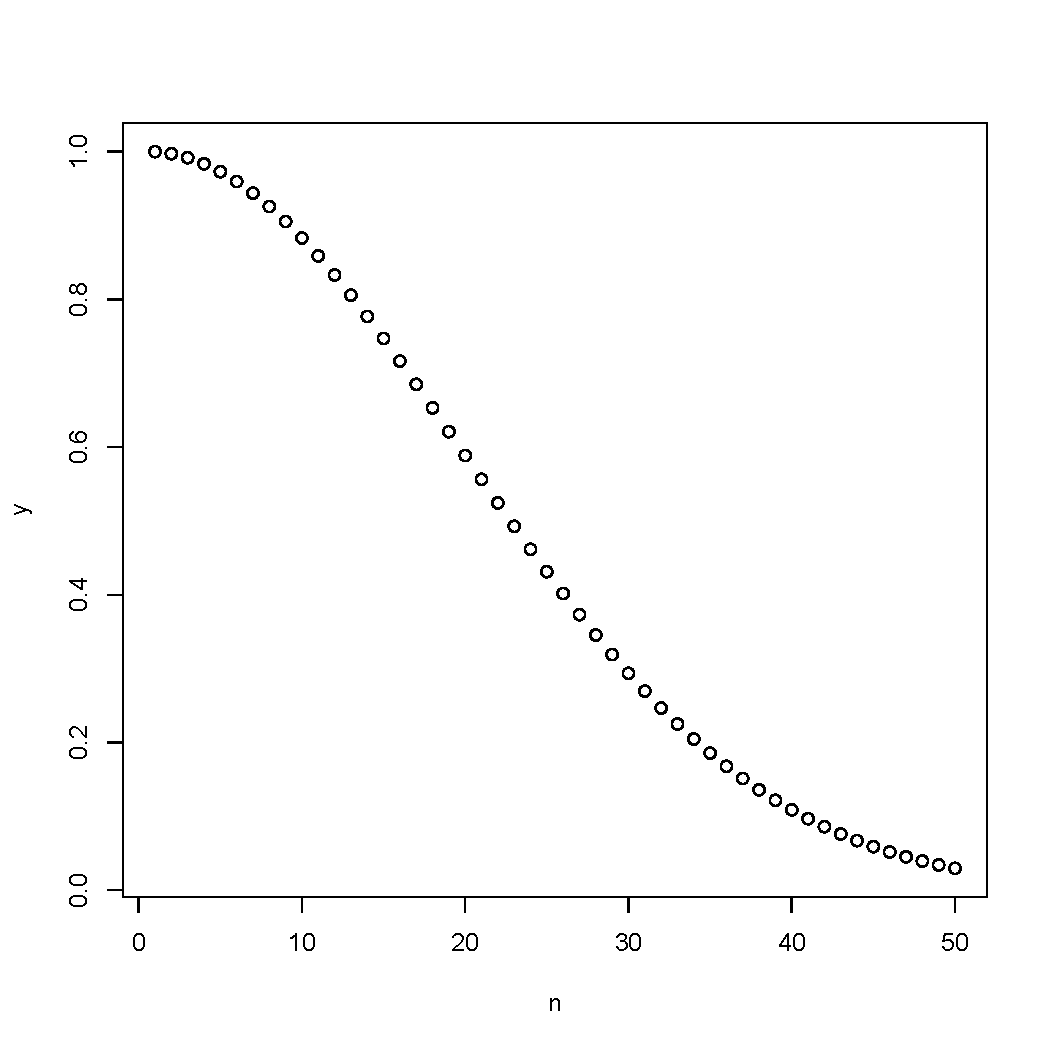
\includegraphics[width=0.85\textwidth]{figures/birthday}
%\end{center}
%}
%
%\vfill
%
%\ct{Nunnikhoven (1992). \textit{A Birthday Problem Solution for Nonuniform Birth Frequencies}.}
%
%\end{frame}



\end{document}
